%
%   Plantilla propuesta de proyectos
%
%
\documentclass{article} 
\usepackage{ASCIDEN_2024B}
\usepackage{graphicx}
\usepackage{amssymb}
\usepackage{ifthen}
\usepackage{hyperref}
\usepackage[utf8]{inputenc}
\usepackage[spanish]{babel}
\begin{document}
\let\tableline=\hline
\let\obs=\sphericalangle

%%%%%%%%%%%%%%%%%%%%%%%%%%%%%%%%%%%%%%%%%%%%%%%%
% Pagina  1
%%%%%%%%%%%%%%%%%%%%%%%%%%%%%%%%%%%%%%%%%%%%%%%%

% Titulo (debe entrar en una sola linea)

\title {Análisis choque Astro-Nubes} 


% Abstract
 
\abstract{ 
Interfaz basada en redes neuronales convolucionales que reconoce colisiones entre nubes de gas y estrellas, entrenadas con datos de simulación, y que determina caracterísitcas clave de la colisión, como lo son la energía del sistema y una posible pérdida de masa de los objetos observados.
}

% Informacion de integrantes  

\pinamea{Francisca Hurtado Morales}                  % Nombre
\piinstitutea{Universidad de Chile}        % Institucion
\pigita{FranciscaHM}           % Usuario de GitHub
\piemaila{franbhm04@gmail.com}                 % Direccion de correo

\pinameb{Martin Minguzzi Aranis}                  % Nombre
\piinstituteb{Universidad de Chile}        % Institucion
\pigitb{mingucci00}           % Usuario de GitHub
\piemailb{martin.minguzzi@ug.uchile.cl}                 % Direccion de correo

\pinamec{Alex Sepulveda Navarrete}                  % Nombre
\piinstitutec{Universidad de Chile}        % Institucion
\pigitc{asgn89}           % Usuario de GitHub
\piemailc{alex.sepulveda.n@ug.uchile.cl}                 % Direccion de correo

\makepgone   % este comando crea la pagina 1




%%%%%%%%%%%%%%%%%%%%%%%%%%%%%%%%%%%%%%%%%%%%%%%%
% Pagina  2
%%%%%%%%%%%%%%%%%%%%%%%%%%%%%%%%%%%%%%%%%%%%%%%%
%
% En esta sección escribe la justificación científica del 
% proyecto. No debe exceder 1 pagina. 
%
\JustificacionCientifica{

En nuestra investigación preliminar acerca de colisiones de galaxias, ricas en gas molecular, significan eventos galácticos de lo mas importantes en la evolución del universo, el correcto análisis de estos fenómenos nos sitúan en escenarios desde "simples" colisiones galácticas hasta investigaciones actuales acerca del protagonismo del gas molecular en interacciones de agujeros negros masivos.\\
El observatorio ALMA ha sido una variable en común que apreciamos en nuestra investigación de proyectos externos y avanzados acerca de estas colisiones, proyectos que están por doquier en la web, es entonces que se refleja la importancia del análisis de estos eventos.\\

Consideramos de los mas interesante y practico estudiar este caso desde un ambiente "seguro" obvio y comodo que son las simulaciones de estos choques, se trata de un análisis desde el factor físico de todo esto, y así, aunque proyecta una aparente abrumadora complejidad, poder trabajar desde un piso estable y conocido que son la física y el manejo de los datos obtenidos a procesar virtualmente con lo aprendido en ciencias de datos.\\

En este escenario se han puesto un montón de científicos de universidades e institutos de renombre tales como Caltech, Harvard y demás.\\

La variedad de artículos científicos que hemos podido abordar abordan el tema de manera distinta, y, desde sus palabras, creen que siguen existiendo muchas mas de hacerlo. Entre estos folletos encontramos una variedad de investigaciones; estudios en Harvard informan mientras avanzan en la noción de la relación entre masividad y abundancia de gas molecular en galaxias y la formación de nuevas estrellas en la resolución de la colisión; por otro lado están los estudios que se limitan al análisis en la observación directa de casos particulares de estos sistemas, apreciando entre estas colisiones en particular la participación de grotescos agujeros negros, como también lo de nuestro interés, enormes nubes gaseosas de gas molecular frio.\\

El análisis de estos sistemas afloja la complejidad del estudio de las interacciones entre estrellas y gas, como también en avanzar en la comprensión de la materia oscura. Con estos análisis podemos lograr entender a pasado, presente y futuro la historia del universo.\\

Como somos parte de esto es obvio que colisiones entre astros tan inconmensurables comparados a nosotros, a nuestra Via Láctea, nos pueden afectar. Y esto es tema de discusión ya que la interacción provoca luz, ondas y un juego de temperaturas que no tendría problema, con la correcta distancia, transferir problemas a futuro en nosotros, si es que ya no lo hizo.\\

Relacionando estudios anteriormente descritos con lo ultimo mencionado en este apartado podemos hacer miles de suposiciones, en las que claro que cabe mencionar de ejemplo la siguiente; sabiendo que descomunales nubes de gases muy lejos de nosotros pueden situarse en el escenario de colisión y resultando así en la formación de incontables estrellas, acorde al tamaño de la nube claro, y la formación de estrellas no se resume en nada menos que la formación de elementos y, producto de la colisión, la distribución a los lugares de la galaxia que correspondan. Asi, situándonos en el peor de los casos quizás la distribución de estos elementos y metales hacia nuestro sistema alteraría para bien o para mal nuestra historia.\\


}


\makepgtwo   % este comando crea la pagina 2

%%%%%%%%%%%%%%%%%%%%%%%%%%%%%%%%%%%%%%%%%%%%%%%%
% Pagina  3
%%%%%%%%%%%%%%%%%%%%%%%%%%%%%%%%%%%%%%%%%%%%%%%%
%
% En esta sección escribe la descripción técnica del proyecto
% propuesto. 
% La descripción se divide en dos partes: los datos a
% utilizar y los métodos (o algoritmos) que se explorarán.
% En los métodos, escribe la idea general de los
% procedimientos propuestos. No debe exceder 1 pagina.
%

\datos{

Datos de simulación de choques entre nubes de gas y estrellas, creados en AMUSE.

}

\bigskip 

\metodos{

Se buscará crear redes neuronales convolucionales (CNN) para detectar las nubes de polvo y estrellas próximas a colisionar. \\
Una vez detectados se medirán los siguientes factores de cada cuerpo antes y después del choque con el fin de conocer las transferencias de energía:\\
\begin{itemize}
\item Temperatura: Para medir la temperatura se deberá tomar en cuenta los colores de cada objeto. Gracias a las imágenes obtenidas podemos realizar una espectroscopía, lo que nos indicará sus líneas de emisión.\\
\item Masa: El análisis de las líneas de emisión nos dará indicios de los componentes de los objetos. Además, las CNN pueden reconocer estructuras para estimar el volumen y así tener una percepción de la densidad del objeto. Con esto podemos analizar las posibles pérdidas de masa ocurridas luego del choque. \\
\item Velocidad: Medir la velocidad de cada objeto, ya sea traslacional o angular, nos entrega información relevante para medir el momentum de los objetos, lo que explicará las estructuras resultantes de estas colisiones.\\
\item Luminosidad: La luminosidad es un aspecto fundamental por medir en este tipo de objetos, ya que directamente nos indica la energía por tiempo de cada objeto. Se debe utilizar fotometría para este tipo de indicadores, por lo que se deberán aplicar filtros fotométricos para las imágenes. Además, debemos de tener en cuenta la distancia a la que se encuentra del observador, ya que su brillo disminuye con el cuadrado de esta.\\
\end{itemize}

 
}

\makepgthree % este comando crea la pagina 3

%%%%%%%%%%%%%%%%%%%%%%%%%%%%%%%%%%%%%%%%%%%%%%%%
% Pagina  4
%%%%%%%%%%%%%%%%%%%%%%%%%%%%%%%%%%%%%%%%%%%%%%%%
%
% Usa esta página para agregar referencias y anexos (figuras
% o tablas) que sean de ayuda en la explicación del proyecto
%

\anexos{ 

% Referencias

\References{References}   
Referencias:

\begin{description}       % Agrega tus referencias siguiendo los ejemplos

 \item Datos Simulación entregados por equipo docente.

 \item 

\end{description}

% Tabla de Ejemplo

\begin{center}
{\bf Tabla 1:} Aca va la leyenda de la tabla. \\
\smallskip
{\small
         \begin{tabular}{lccccr}
            \tableline
            \noalign{\smallskip}
{\rm QSO}&{\rm [Fe/H]}&{\rm [Zn/Fe]}&{\rm [Si/Fe]}&{\rm [S/Fe]}&{\rm Ref.}\\
            \noalign{\smallskip}
            \hline
            \noalign{\smallskip}
Q0149+33   & -1.77  &   0.10  &    0.28 &       ...   &    a,b     \\   
Q0013$-$004& -1.83  &   1.09  &    ...  &       0.79  &    m     \\  

           \noalign{\smallskip}
           \hline

\end{tabular}
}
\end{center}

% Figura de Ejemplo

\center{

   {\bf Figura 1:} Aca va la leyenda de la figura. \\
   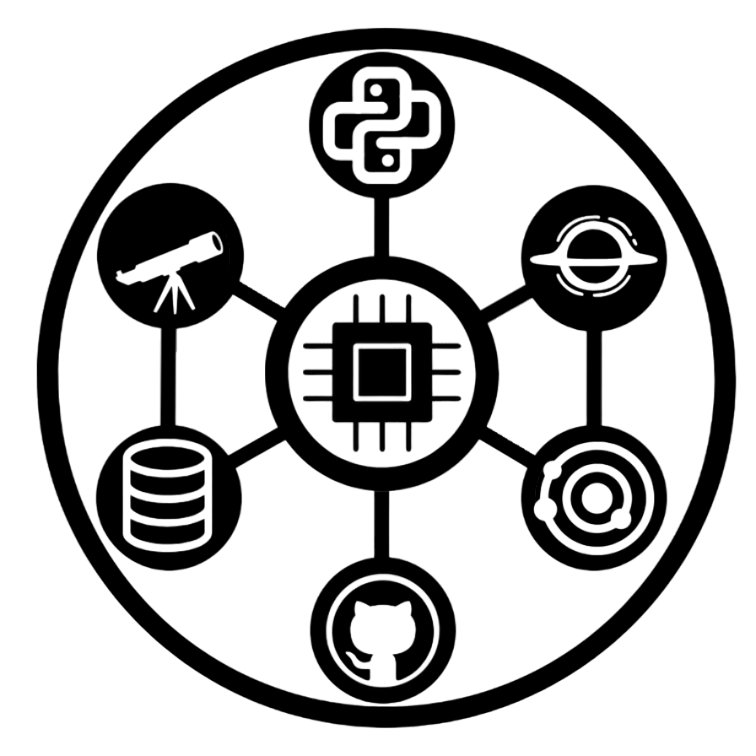
\includegraphics[width=8.5cm,angle=0]{fig1.png}
}


}


\makepgfour   % Este comando crea la pagina 4

\end{document} 

